\clearpage
\appendixsection{Online Description Length of Numerical Probes}
\label{sec:probe-mdl}

\begin{figure*}[t]
\centering
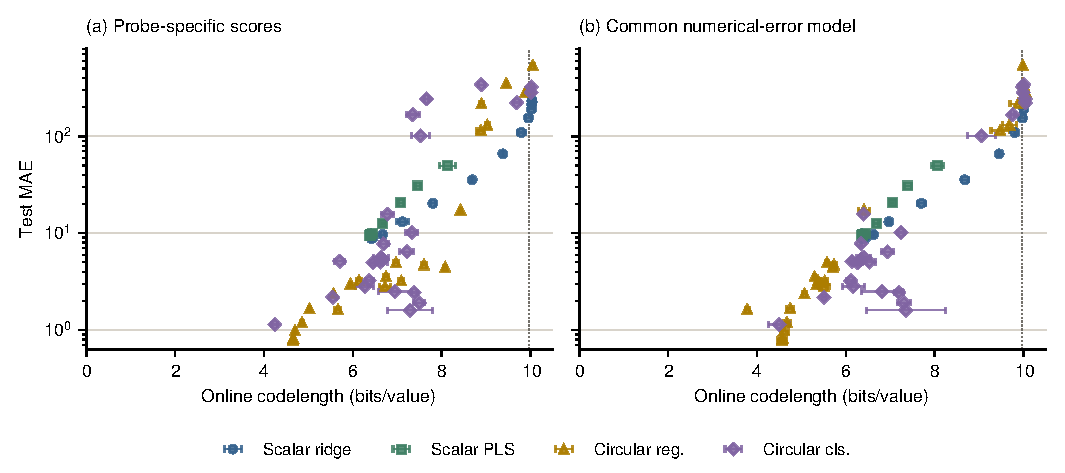
\includegraphics[width=\textwidth]{../figures/fig_probe_mdl.pdf}
\vspace{1mm}
{\small\begin{tabular}{llrrr}
\toprule
Probe & Setting & \multicolumn{2}{c}{Bits/value} & Test MAE \\
 & & Scores & Numerical error & \\
\midrule
Scalar ridge & $\lambda=0$ & 6.41\,$\pm$\,0.01 & 6.37\,$\pm$\,0.04 & 9.83 \\
Scalar PLS & $k=32$ & 6.38\,$\pm$\,0.01 & 6.36\,$\pm$\,0.02 & 9.36 \\
Circular reg. & $d=4096$ & 4.65\,$\pm$\,0.01 & 4.56\,$\pm$\,0.10 & 0.79 \\
Circular reg. & $d=10$ & 5.66\,$\pm$\,0.07 & 3.78\,$\pm$\,0.04 & 1.63 \\
Circular cls. & $d=10$ & 4.24\,$\pm$\,0.07 & 4.50\,$\pm$\,0.24 & 1.14 \\
\bottomrule
\end{tabular}
}
\caption{Circular probes achieve shorter online codes, with relative costs depending on the probability model.
Each panel includes all 73 settings: (a) uses probe-specific scores and (b) a common distribution over numerical errors.
Horizontal whiskers and tabulated $\pm$ values give sample standard deviations across three orderings of the original 800 training labels; test MAE uses separate fits on all 800 training values.
The dotted line marks uniform coding.
The table lists settings minimizing either code: $\lambda$ is the ridge penalty, $k$ the PLS component count, and $d$ the circular-code dimension.
Codelengths are conditional on the agreed setting; the text describes the additional cost of selecting one.}
\label{fig:probe-mdl}
\end{figure*}

A common cost comparison encodes the same numerical labels with each probe.
We fit a probe on labels already transmitted, use its probabilities to encode the next block, and repeat as the fitting sample grows.
This online code \citep{voita2020information} combines predictive accuracy with the ability to learn from limited data.
The coding procedure uses the original 800 training-value centroids of Llama-3.1-8B layer-10 activations (Appendix~\ref{sec:numerical-probe-setup}), with the same 73 settings as Figure~\ref{fig:decodability}d.
Every predictive distribution covers all 1,000 integers from 0 through 999, including values absent from a fitting prefix.
The development and test labels are excluded from coding and calibration.
We evaluate separate fits on all 800 training values using the 100 test values.

\paragraph{Coding procedure.}

The sender and receiver agree on the probe architecture, fitting algorithm, and random seed.
For a shared ordering of the training examples, let $t_1<\cdots<t_K=800$ denote the block boundaries and $q_k$ the distribution fitted using the first $t_k$ examples.
The online codelength is
\begin{align}
 L_{\mathrm{online}} &= t_1\log_2 1000 \notag\\
 &\quad-\sum_{k=1}^{K-1}\sum_{i=t_k+1}^{t_{k+1}}
 \log_2 q_k(v_i\mid h_i),
 \label{eq:probe-online-code}
\end{align}
where $h_i$ is the activation centroid and $v_i$ its numerical label.
Uniform coding supplies the first block.
We follow the fractional schedule of \citet{voita2020information}, rounding down and merging empty or duplicate blocks, giving boundaries
\[
 \{1,3,6,12,25,50,100,200,400,800\}.
\]
The one-label fitting prefix also uses uniform coding for the next block, as it cannot supply both fitting and calibration examples.
We repeat the procedure with ordering seeds 1729, 2718, and 31415, shared across methods.
The uniform reference costs $800\log_2 1000\approx7973$ bits, or 9.97 bits per value.

\paragraph{Probability models.}

For ridge and PLS, the score of candidate value $v$ is $s(v,h)=-(v-\mu(h))^2$, where $\mu(h)$ is the continuous scalar prediction.
Circular regression uses cosine similarity between the predicted and candidate codes; circular classification uses its logits.
We turn these scores into probabilities by temperature scaling and normalization over the common alphabet, mixed with 1\% uniform probability:
\begin{equation}
 q_T(v\mid h)=.99\frac{e^{s(v,h)/T}}{\sum_{u=0}^{999}e^{s(u,h)/T}}+\frac{.01}{1000}.
 \label{eq:probe-mdl-probability}
\end{equation}
An alternative uses $s(v,h)=-|v-\hat v(h)|$, where $\hat v(h)$ is each probe's decoded integer.
This numerical-error distribution applies the same observation model to all four methods.

At each prefix, we reserve its last 20\% of examples, with a minimum of one, for temperature calibration and fit on the rest.
We select the temperature minimizing calibration codelength from 49 logarithmically spaced values between $10^{-6}$ and $10^6$, plus uniform prediction.
The probe is then refitted on the full prefix, keeping that temperature for the next block.
Both parties can reconstruct these choices from labels already transmitted.
PLS components are capped at one less than the number of fitting examples.
The classifier retains its learned 100-dimensional projection, and its early-stopping split uses only its supplied fitting examples.
We reset its initialization seed to 1729 for every fit; the ten-dimensional classifier has test MAE 1.14, compared with 1.09 in Figure~\ref{fig:decodability}d.


\paragraph{Results and interpretation.}

The shortest circular codes use fewer bits than the shortest scalar codes under both probability models (Figure~\ref{fig:probe-mdl}).
With probe-specific scores, the circular minima are 4.24--4.65 bits per value, compared with 6.38--6.41 for scalar probes.
The numerical-error distribution makes circular regression shorter than circular classification, at 3.78 and 4.50 bits per value, respectively.
The ordering within the circular family therefore depends on the distribution used to encode labels.

The plotted costs are conditional on an agreed probe setting.
Selecting one of a family's $M$ settings after observing the message adds $\log_2 M$ bits to communicate that choice.
Here $M$ is 14 for ridge, 11 for PLS, and 24 for each circular method, so this charge is at most 4.59 bits per complete message, or .006 bits per value.
The online code accounts for all learned projections through repeated fitting on already transmitted labels.
Its total cost jointly measures prediction and learning under the specified procedure; it is sensitive to the probability model and calibration choices.

\FloatBarrier
